
In the last three Chapters we have introduced six important \PETSc objects for solving PDEs:
\begin{itemize}
\item[\quad Chapter \ref{chap:ls}:] \pVec, \pMat, \pKSP, \pPC
\item[\quad Chapter \ref{chap:st}:] \pDM\sidenote{In the \pDMDA case only.}
\item[\quad Chapter \ref{chap:nl}:] \pSNES
\end{itemize}
Each example in the rest of the book will use \emph{all} of these object types.

In particular, from now on we will even solve \emph{linear} PDEs using a \pSNES object and Newton iteration.  Linear problems are now merely the case where we know, in advance, that one Newton iteration suffices.  Always using \pSNES gives us uniform code structure and much more flexibility when it comes to changing the PDE problem.

Though we continue with new ideas, in the current Chapter we take a break from using new \PETSc objects.  Instead we first introduce PDEs which arise from minimization in a function space, and then we introduce a structured-grid finite element method (FEM).  Our one example is from an important class of nonlinear PDEs, namely Poisson-like problems with solution-dependent diffusivity.


\section{$p$-Laplacian equation as minimization}

Let $\Omega$ be a domain (connected open subset) in $\RR^2$ or $\RR^3$ with well-behaved boundary.\sidenote{A Lipschitz boundary will suffice in theory.  In practice we use polygonal domains, and merely a rectangle in the current Chapter.}  Consider this nonlinear functional for $p \ge 1$,
\begin{equation}
    I[u] = \int_\Omega \frac{1}{p} |\grad u|^p - fu.  \label{eq:of:functional}
\end{equation}
This functional is well-defined on the Sobolev space \citep{Evans2010} of integrable functions which are defined on $\Omega$ and have integrable gradient, namely
\begin{equation}
    W^{1,p}(\Omega) = \left\{w \,:\, \int_\Omega |w|^p < \infty \,\, \& \, \int_\Omega |\grad w|^p < \infty\right\}, \label{eq:of:sobolevdefn}
\end{equation}
which is a Banach space with norm $\|w\|_{W^{1,p}} = \left(\int_\Omega |w|^p + \int_\Omega |\grad w|^p\right)^{1/p}$.  We will assume that the function $f$ in \eqref{eq:of:functional} is at least integrable, in the sense that $f\in L^q(\Omega)$ for $q$ dual to $p$ (i.e.~ $1/p+1/q=1$), but little is lost if we just consider continuous $f\in C(\Omega)$.

\begin{marginfigure}
\includegraphics[width=1.2\textwidth]{figs/minsurf} % generated by figs/minsurf.tex
\medskip
\caption{The functional $I[u]$ is analogous to the convex surface $z = \tfrac{1}{4}(x^4 + y^4) - 2x + 2y$ shown here, but with input from the $\infty$-dimensional space $W_g^{1,p}(\Omega)$ instead of the plane $\RR^2$.}
\label{fig:of:cartoonfunctional}
\end{marginfigure}

The reader should probably visualize $I[u]$ in \eqref{eq:of:functional} as in our cartoon version Figure \ref{fig:of:cartoonfunctional}.  Not only is it well-defined, but it also has a unique minimum, at least if we add boundary conditions.  To add such conditions we choose a real-valued function $g$ defined along $\partial \Omega$ and we define a subset of $W_g^{1,p}(\Omega)$
\begin{equation}
    W_g^{1,p}(\Omega) = \left\{w \,:\, w \in W^{1,p}(\Omega) \,\, \& \,\, w\big|_{\partial \Omega} = g\right\}.  \label{eq:of:affinedirichlet}
\end{equation}
For this to make sense FIXME

With such Dirichlet boundary conditions, $I[u]$ is \emph{coercive} in the sense that if the norm of the input function from $W_g^{1,p}(\Omega)$ is large then the output is large:
\begin{equation}
\lim_{\|u\|_{W^{1,p}} \to +\infty} I[u] = +\infty.   \label{eq:of:coercivity}
\end{equation}
Secondly it is continuous enough to have a minimum on compact sets, namely it is \emph{weakly lower semi-continuous}, which means, by definition, that
\begin{equation}
\lim_{u\rightharpoonup v} I[u] \ge I[v],  \label{eq:of:lowersemicont}
\end{equation}
where the limit is in the weak topology on $W^{1,p}(\Omega)$ \citep{Evans2010,KinderlehrerStampacchia1980}.  Third it is \emph{convex}, meaning
\begin{equation}
I[\lambda u + (1-\lambda) v] \le \lambda I[u] + (1-\lambda) I[v]    \label{eq:of:convexity}
\end{equation}
if $u,v\in W^{1,p}(\Omega)$ and $0 \le \lambda \le 1$.  \citet{KinderlehrerStampacchia1980} show that the three properties \eqref{eq:of:coercivity}, \eqref{eq:of:lowersemicont}, \eqref{eq:of:convexity} imply that the problem
\begin{equation}
\min_{u \in W_g^{1,p}(\Omega)} I[u] \label{eq:of:plapmin}
\end{equation}
has a unique solution.

On the other hand, the solution to this minimization problem is also the solution to a nonlinear PDE.  Indeed, if $p>1$ then the functional $I[u]$ is smooth enough to have a gradient (derivative).  The statement that the gradient is zero at the minimum has several names, among them \emph{variational equation}, \emph{Euler-Lagrange equation}, and the \emph{weak form} of the PDE.  The multiple names suggest the centrality of the following calculation to many parts of applied mathematics.

Assume $\eps$ is a real number and $u,v \in W^{1,p}(\Omega)$.  Then
\begin{align*}
I[u+\eps v] - I[u] &= \int_\Omega \frac{1}{p} |\grad u + \eps \grad v|^p + \frac{1}{p} |\grad u|^p - \eps f v \\
   &= \eps \left(\int_\Omega |\grad u|^{p-2} \grad u \cdot \grad v - f v\right) + O(\eps^2),
\end{align*}
and so the gradient exists,
\begin{equation}
\grad I[u](v) = \lim_{\eps\to 0} \frac{I[u+\eps v] - I[u]}{\eps} = \int_\Omega |\grad u|^{p-2} \grad u \cdot \grad v - f v, \label{eq:of:plapfunctionalderivative}
\end{equation}
defining a map $\grad I[u] : W^{1,p}(\Omega) \to \RR$ for each $u \in W^{1,p}(\Omega)$.  If $u$ solves \eqref{eq:of:plapmin} and $v\in W_0^{1,p}(\Omega)$ then $\grad I[u](v)=0$ or
\begin{equation}
\int_\Omega |\grad u|^{p-2} \grad u \cdot \grad v - f v = 0. \label{eq:of:plapweakform}
\end{equation}
From now on we refer to \eqref{eq:of:plapweakform} as the \emph{weak form} of the $p$-\emph{Laplacian} equation.

FIXME this becomes a \emph{strong form}, the traditional form of the $p$-Laplacian equation by another integration by parts,
\begin{equation}
- \Div\left(|\grad u|^{p-2} \grad u\right) = f
\label{eq:of:plapstrongform}
\end{equation}
which is \eqref{poissonsquare} if $p=2$


\section{Structured $Q^1$ finite elements}

FIXME show grid with $(i,j)$ indexing on nodes, and $\ell=0,1,2,3$ indexing on corners of element $\square_{i,j}$

FIXME show bilinear functions and their basis $\chi_\ell(\xi,\eta)$ on reference element $\square_\ast = [-1,1]\times[-1,1]$

FIXME hat functions
    $$\psi_{i,j}(x_r,y_s) = \delta_{ir} \delta_{js}$$

\begin{marginfigure}
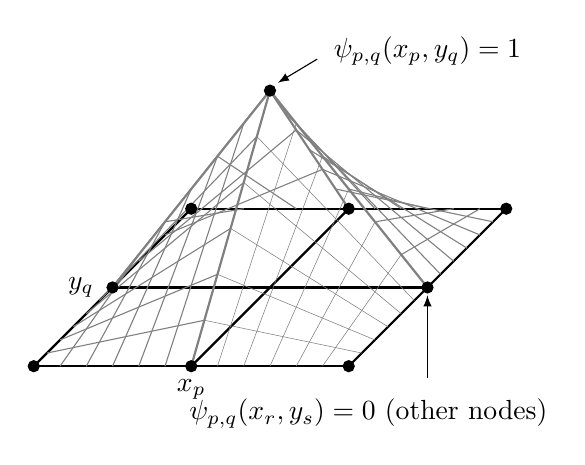
\begin{tikzpicture}[scale=0.5]

  % strong grid around elements
  \draw[thick] (0,0) -- (8,0);
  \draw[thick] (2,2) -- (10,2);
  \draw[thick] (4,4) -- (12,4);
  \draw[thick] (0,0) -- (4,4);
  \draw[thick] (4,0) -- (8,4);
  \draw[thick] (8,0) -- (12,4);

  \def\ytop{7};

  % tent lines
  \draw[gray,thick] (6,\ytop) -- (4,0);
  \draw[gray,thick] (6,\ytop) -- (2,2);
  \draw[gray,thick] (6,\ytop) -- (10,2);
  \draw[gray,thick] (6,\ytop) -- (8,4);

  \def\dx{(10.0-6.0)/6};
  \def\dy{(2.0-\ytop)/6};
  \foreach \jj in {1,...,5}
  {
       \draw[gray,very thin] ({6+\jj*\dx},{\ytop+\jj*\dy}) -- ({4+(4/6)*\jj},0.0);
  }

  \def\dx{(4.0-6.0)/6};
  \def\dy{(0.0-\ytop)/6};
  \foreach \jj in {1,...,5}
  {
       \draw[gray,very thin] ({6+\jj*\dx},{\ytop+\jj*\dy}) -- ({10-(2/6)*\jj},{2-(2/6)*\jj});
  }

  \def\dx{(2.0-6.0)/6};
  \def\dy{(2.0-\ytop)/6};
  \foreach \jj in {1,...,5}
  {
       \draw[gray,thin] ({6+\jj*\dx},{\ytop+\jj*\dy}) -- ({4-(4/6)*\jj},0.0);
  }

  \def\dx{(4.0-6.0)/6};
  \def\dy{(0.0-\ytop)/6};
  \foreach \jj in {1,...,5}
  {
       \draw[gray,thin] ({6+\jj*\dx},{\ytop+\jj*\dy}) -- ({2-(2/6)*\jj},{2-(2/6)*\jj});
  }

  \def\dx{(10.0-6.0)/6};
  \def\dy{(2.0-\ytop)/6};
  \foreach \jj in {1,...,5}
  {
       \draw[gray,thin] ({6+\jj*\dx},{\ytop+\jj*\dy}) -- ({8+(4/6)*\jj},4.0);
  }

  \def\dx{(8.0-6.0)/6};
  \def\dy{(4.0-\ytop)/6};
  \foreach \jj in {1,...,5}
  {
       \draw[gray,thin] ({6+\jj*\dx},{\ytop+\jj*\dy}) -- ({10+(2/6)*\jj},{2+(2/6)*\jj});
  }

  \def\dx{(2.0-6.0)/3};
  \def\dy{(2.0-\ytop)/3};
  \foreach \jj in {1,...,2}  % reduce clutter
  {
       \draw[gray,thin] ({6+\jj*\dx},{\ytop+\jj*\dy}) -- ({8-(4/3)*\jj},4.0);
  }

  \def\dx{(8.0-6.0)/3};
  \def\dy{(4.0-\ytop)/3};
  \foreach \jj in {1,...,2}
  {
       \draw[gray,thin] ({6+\jj*\dx},{\ytop+\jj*\dy}) -- ({2+(2/3)*\jj},{2+(2/3)*\jj});
  }

  % nodes in base plane
  \filldraw (0,0) circle (4pt);
  \filldraw (4,0) circle (4pt);
  \filldraw (8,0) circle (4pt);
  \filldraw (2,2) circle (4pt);
  %\filldraw (6,2) circle (4pt);   % (x_j,y_k) is at (6,2)
  \filldraw (10,2) circle (4pt);
  \filldraw (4,4) circle (4pt);
  \filldraw (8,4) circle (4pt);
  \filldraw (12,4) circle (4pt);

  % node at tent top
  \filldraw (6,\ytop) circle (4pt);

  % annotate
  \draw (10,\ytop+1.0) node {$\psi_{p,q}(x_p,y_q)=1$};
  \draw[-latex] (7.2,\ytop+0.8) -- (6.2,\ytop+0.2);
  \draw (8.5,-1.2) node {$\psi_{p,q}(x_r,y_s)=0$ (other nodes)};
  \draw[-latex] (10,-0.3) -- (10,1.8);

  % label center point
  \draw (4,-0.6) node {$x_p$};
  \draw (1.2,2) node {$y_q$};

\end{tikzpicture}

\caption{FIXME}
\label{fig:q1hat}
\end{marginfigure}


\section{Implementation with objective only}

FIXME code uses \texttt{SNESSetObjective()} only, though also \texttt{SNESSetFunction()}; no hand-made Jacobian at all

FIXME try NCG

\cinputpart{plap.c}{\CODELOC}{FIXME I}{I}{//STARTCONFIGURE}{//ENDCONFIGURE}{code:plapI}

\cinputpart{plap.c}{\CODELOC}{FIXME II}{II}{//STARTEXACTF}{//ENDEXACTF}{code:plapII}

\cinputpart{plap.c}{\CODELOC}{FIXME III}{III}{//STARTOBJECTIVE}{//ENDOBJECTIVE}{code:plapIII}

\cinputpart{plap.c}{\CODELOC}{FIXME IV}{IV}{//STARTMAIN}{//ENDMAIN}{code:plapIV}


\section{Residual function $=$ gradient}

\cinputpart{plap.c}{\CODELOC}{FIXME V}{V}{//STARTFUNCTION}{//ENDFUNCTION}{code:plapV}


\section{Exercises}

\renewcommand{\labelenumi}{\arabic{chapter}.\arabic{enumi}\quad}
\renewcommand{\labelenumii}{(\alph{enumii})}
\begin{enumerate}
\item Prove coercivity \eqref{eq:of:coercivity} and convexity \eqref{eq:of:convexity} of functional $I[u]$ defined in \eqref{eq:of:functional}.  The finite dimensional facts that FIXME for $\xi,\eta\in\RR^n$ will be useful.
\item FIXME
\end{enumerate}